\chapter{Vergleich}
\label{chap:vergleich}
In diesem Kapitel werden numerische Ergebnisse
der beiden Verfahren f�r verschiedene Testprobleme
vorgestellt.
Der Test wird auf Optimierungsprobleme
mit linearen Restriktionen beschr�nkt, d.\,h.,
Optimierungsprobleme mit nichtlinearen Restriktionen
werden wegen des hohen Aufwands
nicht ber�cksichtigt.

\section{Testprobleme}
\label{sec:testprobleme}
Die Testprobleme k�nnen in drei Gruppen geteilt werden.
Die erste Gruppe besteht aus Problemen
\eqref{prob:opt_prob_mit_var_beschr}
mit nur oberen und unteren Schranken.
Zu der zweiten Gruppe geh�ren die Probleme
\eqref{prob:opt_prob_mit_lin_gl_nebenbed}
mit linearen Gleichungsnebenbedingungen.
Die Probleme \eqref{prob:opt_prob_mit_lin_ungl_nebenbed}
mit linearen Ungleichungsnebenbedingungen
kommen anschlie�end in die letzte Gruppe.
In jeder Beschreibung der Testprobleme
werden der zu verwendende Startpunkt $x^0$
und die L�sung $\xopt$ auch angegeben.
\begin{testproblem}
\label{test_prob:prob_v_quad_func}
\begin{gather}
\min_{x\in\R^2}\ (x_1 - 4)^2 + (x_2 - 7)^2 \notag \\
\begin{split}
\nb -10 \leq x_i & \leq 10,\ i = 1,2 \\
\end{split}
\end{gather}
\begin{equation*}
x^0 = (8, 9)^T \quad\text{und}\quad \xopt = (4, 7)^T.
\end{equation*}
\end{testproblem}

\begin{testproblem}
(Rosenbrock-Funktion, vgl. Beispiel 1.4.1 in \cite[S.~14]{alt})
\begin{gather}
\min_{x\in\R^2}\ 100 (x_2-x_1^2)^2+(1-x_1)^2  \notag \\
\begin{split}
\nb -10 \leq x_i & \leq 10,\ i = 1,2 \\
\end{split}
\end{gather}
\begin{equation*}
x^0 = (-1, 2)^T \quad\text{und}\quad \xopt = (1, 1)^T.
\end{equation*}
\end{testproblem}

\begin{figure}[h]
  \centering
  \includegraphics[width=0.45\textwidth]{rosenbrock}
  \includegraphics[width=0.45\textwidth]{himmelblau}
  \caption{Rosenbrock- und Himmelblau-Funktion}
  \label{fig:rosenbrock_und_himmelblau}
\end{figure}

\begin{testproblem}
(Himmelblau-Funktion, vgl. Beispiel 1.4.2 in \cite[S.~14~f.]{alt})
\begin{gather}
\min_{x\in\R^2}\ (x_1^2+x_2-11)^2 + (x_1+x_2^2-7)^2  \notag \\
\begin{split}
\nb -10 \leq x_i & \leq 10,\ i = 1,2 \\
\end{split}
\end{gather}
\begin{equation*}
x^0 = (5, 5)^T \quad\text{und}\quad \xopt = (3, 2)^T.
\end{equation*}
\end{testproblem}

\begin{testproblem}
(Bazaraa-Shetty-Funktion, vgl. Beispiel 1.4.3 in \cite[S.~15~f.]{alt})
\begin{gather}
\min_{x\in\R^2}\ (x_1-2)^4+(x_1-2 x_2)^2  \notag \\
\begin{split}
\nb -10 \leq x_i & \leq 10,\ i = 1,2 \\
\end{split}
\end{gather}
\begin{equation*}
x^0 = (5, 5)^T \quad\text{und}\quad \xopt = (2, 1)^T.
\end{equation*}
\end{testproblem}

\begin{testproblem}
(Beale-Funktion, vgl. Aufgabe 2.2 in \cite[S.~39]{alt})
\begin{gather}
\min_{x\in\R^2}\ (1.5-x_1 (1-x_2))^2+(2.25-x_1 (1-x_2^2))^2+(2.625-x_1 (1-x_2^3))^2  \notag \\
\begin{split}
\nb -10 \leq x_i & \leq 10,\ i = 1,2 \\
\end{split}
\end{gather}
\begin{equation*}
x^0 = (5, 0)^T \quad\text{und}\quad \xopt = (3, 0.5)^T.
\end{equation*}
\end{testproblem}

\begin{testproblem}
(Exponent-Funktion)
\begin{gather}
\min_{x\in\R^2}\ e^{\|x\|^2} \notag \\
\begin{split}
\nb -10 \leq x_i & \leq 10,\ i = 1,2 \\
\end{split}
\end{gather}
\begin{equation*}
x^0 = (5, 4)^T \quad\text{und}\quad \xopt = (0, 0)^T.
\end{equation*}
\end{testproblem}

\begin{figure}[h]
  \centering
  \includegraphics[width=0.45\textwidth]{bazaraa-shetty}
  \includegraphics[width=0.45\textwidth]{exp-func}
  \caption{Bazaraa-Shetty- und Exponent-Funktion}
  \label{fig:bazaraa_shetty_und_exp_funktion}
\end{figure}

\begin{testproblem}
\begin{gather}
\begin{split}
  \min_{x\in\R^4}\ & 100(x_2-x_1^2)^2 + (1-x_1)^2 + 90(x_4-x_3^2)^2 + (1-x_3)^2\\
    & + 10.1((x_2-1)^2 + (x_4-1)^2) + 19.8(x_2-1)(x_4-1)
\end{split} \notag \\
\begin{split}
\nb -10 \leq x_i & \leq 10,\ i = 1,\ldots,4 \\
\end{split}
\end{gather}
\begin{equation*}
x^0 = (3, -1, -3, -1)^T \quad\text{und}\quad \xopt = (1, 1, 1, 1)^T.
\end{equation*}
\end{testproblem}

\begin{testproblem}
(Dixon-Funktion, vgl. Beispiel 1.4.5 in \cite[S.~16]{alt})
\begin{gather}
\min_{x\in\R^{10}}\ (1-x_1)^2 + \sum_{k=1}^{9} (x_k^2-x_{k+1})^2 + (1-x_{10})^2 \notag \\
\begin{split}
\nb -10 \leq x_i & \leq 10,\ i = 1,\ldots,10 \\
\end{split}
\end{gather}
\begin{equation*}
x^0 = (10, \ldots, 10)^T \quad\text{und}\quad \xopt = (1, \ldots, 1)^T.
\end{equation*}
\end{testproblem}

\begin{testproblem}
\begin{gather}
\min_{x\in\R^3}\ (x_1 - 4)^2 + (x_2 - 2)^2 + (x_3 - 7)^2 \notag \\
\begin{split}
\nb 5 \leq x_i & \leq 10,\ i = 1,2,3 \\
\end{split}
\end{gather}
\begin{equation*}
x^0 = (7, 10, 9)^T \quad\text{und}\quad \xopt = (5, 5, 7)^T.
\end{equation*}
\end{testproblem}

\begin{testproblem}
(Rosenbrock-Funktion)
\begin{gather}
\min_{x\in\R^2}\ 100 (x_2-x_1^2)^2+(1-x_1)^2  \notag \\
\begin{split}
\nb -10 \leq x_1 & \leq 10 \\
1.5 \leq x_2 & \leq 10 \\
\end{split}
\end{gather}
\begin{equation*}
x^0 = (2, 3)^T \quad\text{und}\quad \xopt = (1.224, 1.5)^T.
\end{equation*}
\end{testproblem}

\begin{testproblem}
(Himmelblau-Funktion)
\begin{gather}
\min_{x\in\R^2}\ (x_1^2+x_2-11)^2 + (x_1+x_2^2-7)^2  \notag \\
\begin{split}
\nb -10 \leq x_1 & \leq 10 \\
5 \leq x_2 & \leq 10 \\
\end{split}
\end{gather}
\begin{equation*}
x^0 = (10, 10)^T \quad\text{und}\quad \xopt = (-2.928, 5)^T.
\end{equation*}
\end{testproblem}

\begin{testproblem}
(Bazaraa-Shetty-Funktion)
\begin{gather}
\min_{x\in\R^2}\ (x_1-2)^4+(x_1-2 x_2)^2  \notag \\
\begin{split}
\nb 4 \leq x_1 & \leq 10 \\
-10 \leq x_2 & \leq 10 \\
\end{split}
\end{gather}
\begin{equation*}
x^0 = (7, 5)^T \quad\text{und}\quad \xopt = (4, 2)^T.
\end{equation*}
\end{testproblem}

\begin{testproblem}
\label{test_prob:prob_v_beale_1}
(Beale-Funktion)
\begin{gather}
\min_{x\in\R^2}\ (1.5-x_1 (1-x_2))^2+(2.25-x_1 (1-x_2^2))^2+(2.625-x_1 (1-x_2^3))^2  \notag \\
\begin{split}
\nb 3 \leq x_1 & \leq 10 \\
-10 \leq x_2 & \leq 10 \\
\end{split}
\end{gather}
\begin{equation*}
x^0 = (5, 0)^T \quad\text{und}\quad \xopt = (3, 0.5)^T.
\end{equation*}
\end{testproblem}

\begin{testproblem}
(Exponent-Funktion)
\begin{gather}
\min_{x\in\R^3}\ e^{\|x\|^2} \notag \\
\begin{split}
\nb 0.5 \leq x_1 & \leq 10 \\
1 \leq x_2 & \leq 10 \\
1 \leq x_3 & \leq 10 \\
\end{split}
\end{gather}
\begin{equation*}
x^0 = (5, 2, 4)^T \quad\text{und}\quad \xopt = (0.5, 1, 1)^T.
\end{equation*}
\end{testproblem}

\begin{testproblem}
\begin{gather}
\begin{split}
  \min_{x\in\R^4}\ & 100(x_2-x_1^2)^2 + (1-x_1)^2 + 90(x_4-x_3^2)^2 + (1-x_3)^2\\
    & + 10.1((x_2-1)^2 + (x_4-1)^2) + 19.8(x_2-1)(x_4-1)
\end{split} \notag \\
\begin{split}
\nb 2 \leq x_1 & \leq 10 \\
-10 \leq x_2 & \leq 10 \\
-10 \leq x_3 & \leq 10 \\
-10 \leq x_4 & \leq 10 \\
\end{split}
\end{gather}
\begin{equation*}
x^0 = (3, -1, -3, -1)^T \quad\text{und}\quad \xopt = (2, 3.831, 0.03, -0.178)^T.
\end{equation*}
\end{testproblem}

\begin{testproblem}
(Dixon-Funktion)
\begin{gather}
\min_{x\in\R^{10}}\ (1-x_1)^2 + \sum_{k=1}^{9} (x_k^2-x_{k+1})^2 + (1-x_{10})^2 \notag \\
\begin{split}
\nb 2 \leq x_i & \leq 10,\ i = 1,\ldots,10 \\
\end{split}
\end{gather}
\begin{equation*}
x^0 = (10, \ldots, 10)^T \quad\text{und}\quad \xopt = (2, \ldots, 2, 2.5)^T.
\end{equation*}
\end{testproblem}

\begin{testproblem}
\label{test_prob:lin_regres}
Lineare Regression (Vgl. Beispiel~\ref{example:lineare_regression}
auf Seite~\pageref{example:lineare_regression})
\begin{gather}
\min_{x\in\R^2}\ \sum_{i=1}^{10} (x_1 \xi_i + x_2 - \eta_i)^2 \notag \\
\begin{split}
\nb -10 \leq x_i & \leq 10,\ i = 1,2 \\
\end{split}
\end{gather}
\begin{equation*}
x^0 = (-10, 10)^T.
\end{equation*}

Die Messwerte $(\xi_i,\eta_i), i = 1,\ldots,10,$
sind in der Tabelle~\ref{tbl:messwerte_lin_regres}
zu finden.
\begin{equation*}
\xopt = (0.7, -4.3)^T
\quad \Rightarrow \quad
\tilde{\eta}(\xi) = 0.7\, \xi - 4.3 \,.
\end{equation*}
\end{testproblem}

\begin{table}[h]
\centering
\begin{tabular*}{0.8\linewidth}{@{\extracolsep{\fill}}c|cccccccccc}
  $\xi_i$ & 1 & 2 & 3 & 4 & 5 & 6 & 7 & 8 & 9 & 10 \\
  \midrule
  $\eta_i$ & $-0.5$ & $-2$ & $-3$ & $-3$ & $-2.5$
    & $-2$ & $-1$ & 1 & 3 & $5.5$ \\
\end{tabular*}
\caption{Messwerte f�r Testprobleme~\ref{test_prob:lin_regres}
und~\ref{test_prob:nichtlin_regres_quad}}
\label{tbl:messwerte_lin_regres}
\end{table}

\begin{testproblem}
\label{test_prob:nichtlin_regres_quad}
Nichtlineare Regression mit dem funktionalen
Zusammenhang~\eqref{eq:nichtlin_regres_quad_zusammenhang}
(Vgl. Beispiel~\ref{example:nichtlineare_regression}
auf Seite~\pageref{example:nichtlineare_regression})
\begin{gather}
\min_{x\in\R^3}\ \sum_{i=1}^{10} (x_1 (\xi_i -x_2)^2 + x_3 - \eta_i)^2 \notag \\
\begin{split}
\nb -10 \leq x_i & \leq 20,\ i = 1,2,3 \\
\end{split}
\end{gather}
\begin{equation*}
x^0 = (1, 3, -4)^T.
\end{equation*}

Die Messwerte
in der Tabelle~\ref{tbl:messwerte_lin_regres}
sind zu benutzen.
\begin{equation*}
\xopt = (0.242, 4.056, -2.955)^T
\quad \Rightarrow \quad
\hat{\eta}(\xi) = 0.242\, (\xi - 4.056)^2 - 2.955 \,.
\end{equation*}
\end{testproblem}

\begin{figure}[h]
\centering
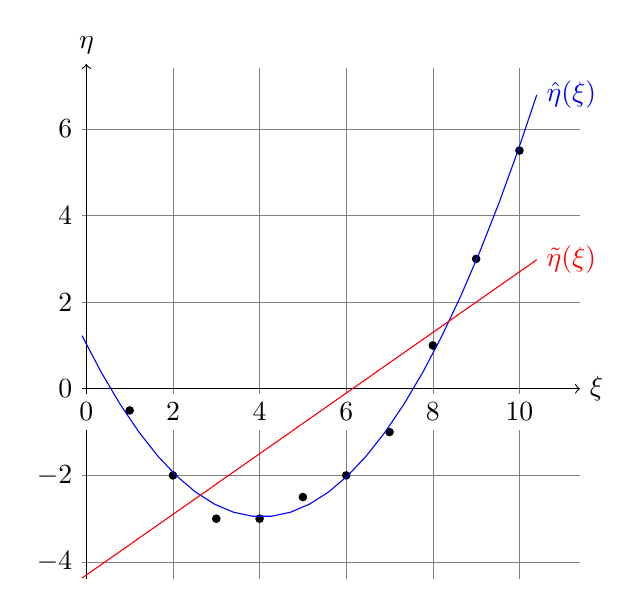
\begin{tikzpicture}[domain=-0.1:10.4,scale=0.55]
  \draw[very thin,color=gray,step=2] (-0.1,-4.4) grid (11.4,7.4);
  \draw[->] (-0.1,0) -- (11.4,0) node[right] {$\xi$};
  \draw[->] (0,-4.4) -- (0,7.5) node[above] {$\eta$};
  %\draw (-0.1,0.2) node [below left,fill=white] {0};
  \foreach \x in {0,2,4,...,10}
    \draw (\x,-0.1) node[below,fill=white] {$\x$};
  \foreach \y in {-4,-2,...,6}
    \draw (-0.1,\y) node[left] {$\y$};
  \foreach \x/\y in
    {1/-0.5, 2/-2, 3/-3, 4/-3, 5/-2.5, 6/-2, 7/-1, 8/1, 9/3, 10/5.5}
    \fill (\x,\y) circle(0.1);
  \draw[color=blue] plot (\x,{0.242*(\x-4.056)^2-2.955})
    node[right] {$\hat{\eta}(\xi)$};
  \draw[color=red] plot (\x,{0.7*\x-4.3})
    node[right] {$\tilde{\eta}(\xi)$};
\end{tikzpicture}
\caption{Ergebnisse der Testprobleme~\ref{test_prob:lin_regres}
und~\ref{test_prob:nichtlin_regres_quad}}
\end{figure}

\begin{testproblem}
\label{test_prob:nichtlin_regres_exp}
Nichtlineare Regression mit dem funktionalen
Zusammenhang~\eqref{eq:nichtlin_regres_exp_zusammenhang}
(Vgl. Beispiel~\ref{example:nichtlineare_regression}
auf Seite~\pageref{example:nichtlineare_regression})
\begin{gather}
\min_{x\in\R^2}\ \sum_{i=1}^{10} (x_1 e^{\xi x_2} - \eta_i)^2 \notag \\
\begin{split}
\nb -10 \leq x_i & \leq 10,\ i = 1,2 \\
\end{split}
\end{gather}
\begin{equation*}
x^0 = (0.2, 0.5)^T.
\end{equation*}

Die Messwerte $(\xi_i,\eta_i), i = 1,\ldots,10,$
sind in der Tabelle~\ref{tbl:messwerte_nichtlin_regres}
gegeben.
\begin{equation*}
\xopt = (0.632, 0.195)^T
\quad \Rightarrow \quad
\bar{\eta}(\xi) = 0.632\, e^{0.195\,\xi}.
\end{equation*}
\end{testproblem}

\begin{table}[h]
\centering
\begin{tabular*}{0.8\linewidth}{@{\extracolsep{\fill}}c|cccccccccc}
  $\xi_i$ & 1 & 2 & 3 & 4 & 5 & 6 & 7 & 8 & 9 & 10 \\
  \midrule
  $\eta_i$ & 1 & 1.1 & 1.2 & 1.35 & 1.55
    & 1.75 & 2.5 & 3 & 3.7 & 4.5 \\
\end{tabular*}
\caption{Messwerte f�r Testproblem~\ref{test_prob:nichtlin_regres_exp}}
\label{tbl:messwerte_nichtlin_regres}
\end{table}

\begin{testproblem}
(vgl. Beispiel 16.2 in \cite[S.~452]{nocedal}
\begin{equation}
\min_{x\in\R^3}\ 3 x_1^2 + 2 x_1 x_2 + x_1 x_3 + 2.5 x_2^2 + 2 x_2 x_3 + 2 x_3^2 - 8 x_1 - 3 x_2 - 3 x_3
\end{equation}
\begin{equation*}
\begin{split}
\nb x_1 + x_3 & = 3 \\
x_2 + x_3 & = 0 \\
\end{split}
\end{equation*}
\end{testproblem}

\begin{testproblem}
\begin{equation}
\min_{x\in\R^5}\ \| x \|^2
\end{equation}
\begin{equation*}
\begin{split}
\nb x_1 + x_2 + x_3 + x_4 + x_5 & = 1 \\
\end{split}
\end{equation*}
\end{testproblem}

\begin{testproblem}
(vgl. Problem 28 in \cite[S.~51]{hock})
\begin{equation}
\min_{x\in\R^3}\ (x_1 + x_2)^2 + (x_2 + x_3)^2
\end{equation}
\begin{equation*}
\begin{split}
\nb x_1 + 2 x_2 + 3 x_3 & = 1 \\
\end{split}
\end{equation*}
\end{testproblem}

\begin{testproblem}
(vgl. Problem 48 in \cite[S.~71]{hock})
\begin{equation}
\min_{x\in\R^5}\ (x_1 - 1)^2 + (x_2 - x_3)^2 + (x_4 - x_5)^2
\end{equation}
\begin{equation*}
\begin{split}
\nb x_1 + x_2 + x_3 + x_4 + x_5 & = 5 \\
x_3 - 2 x_4 - 2 x_5 & = -3 \\
\end{split}
\end{equation*}
\end{testproblem}

\begin{testproblem}
(vgl. Problem 51 in \cite[S.~74]{hock})
\begin{equation}
\min_{x\in\R^5}\ (x_1 - x_2)^2 + (x_2 + x_3 - 2)^2 + (x_4 - 1)^2 + (x_5 - 1)^2
\end{equation}
\begin{equation*}
\begin{split}
\nb x_1 + 3 x_2 & = 4 \\
x_3 + x_4 - 2 x_5 & = 0 \\
x_2 - x_5 & = 0 \\
\end{split}
\end{equation*}
\end{testproblem}

\begin{testproblem}
(vgl. Problem 52 in \cite[S.~75]{hock})
\begin{equation}
\min_{x\in\R^5}\ (4 x_1 - x_2)^2 + (x_2 + x_3 - 2)^2 + (x_4 - 1)^2 + (x_5 - 1)^2
\end{equation}
\begin{equation*}
\begin{split}
\nb x_1 + 3 x_2 & = 0 \\
x_3 + x_4 - 2 x_5 & = 0 \\
x_2 - x_5 & = 0 \\
\end{split}
\end{equation*}
\end{testproblem}

\begin{testproblem}
(vgl. Problem 53 in \cite[S.~76]{hock})
\begin{equation}
\min_{x\in\R^5}\ (x_1 - x_2)^2 + (x_2 + x_3 - 2)^2 + (x_4 - 1)^2 + (x_5 - 1)^2
\end{equation}
\begin{equation*}
\begin{split}
\nb x_1 + 3 x_2 & = 0 \\
x_3 + x_4 - 2 x_5 & = 0 \\
x_2 - x_5 & = 0 \\
-10 \leq x_i & \leq 10,\ i = 1,\ldots,5 \\
\end{split}
\end{equation*}
\end{testproblem}

\begin{testproblem}
(vgl. Problem 49 in \cite[S.~72]{hock})
\begin{equation}
\min_{x\in\R^5}\ (x_1-x_2)^2 + (x_3-1)^2 + (x_4-1)^2 + (x_5-1)^6 
\end{equation}
\begin{equation*}
\begin{split}
\nb x_1 + x_2 + x_3 + 4 x_4 & = 7 \\
x_3 + 5 x_5 & = 6 \\
\end{split}
\end{equation*}
\end{testproblem}

\begin{testproblem}
(vgl. Problem 50 in \cite[S.~73]{hock})
\begin{equation}
\min_{x\in\R^5}\ (x_1-x_2)^2 + (x_2-x_3)^2 + (x_3-x_4)^4 + (x_4-x_5)^2 
\end{equation}
\begin{equation*}
\begin{split}
\nb x_1 + 2 x_2 + 3 x_3 & = 6 \\
x_2 + 2 x_3 + 3 x_4 & = 6 \\
x_3 + 2 x_4 + 3 x_5 & = 6 \\
\end{split}
\end{equation*}
\end{testproblem}

\begin{testproblem}
\begin{equation}
\min_{x\in\R^2}\ x_1^2 + x_2^2 - 4 x_1 - 4 x_2
\end{equation}
\begin{equation*}
\begin{split}
\nb 2 x_1 + x_2 & \leq 2 \\
x_1 - x_2 & \leq 1 \\
-x_1 - x_2 & \leq 1 \\
-2 x_1 + x_2 & \leq 2 \\
\end{split}
\end{equation*}
\end{testproblem}

\begin{testproblem}
(vgl. Beispiel 16.4 in \cite[S.~475]{nocedal})
\begin{equation}
\min_{x\in\R^2}\ (x_1 - 1)^2 + (x_2 - 2.5)^2
\end{equation}
\begin{equation*}
\begin{split}
\nb -x_1 + 2 x_2 & \leq 2 \\
x_1 + 2 x_2 & \leq 6 \\
x_1 - 2 x_2 & \leq 2 \\
0 & \leq x_i,\ i = 1,2 \\
\end{split}
\end{equation*}
\end{testproblem}

\begin{testproblem}
(vgl. Beispiel 13.2 in \cite[S.~415f]{antoniou})
\begin{equation}
\min_{x\in\R^4}\ (x_1 - x_3)^2 + (x_2 - x_4)^2
\end{equation}
\begin{equation*}
\begin{split}
\nb -x_1 & \leq 0 \\
-x_2 & \leq 0 \\
x_1 + 2 x_2 & \leq 2 \\
-x_4 & \leq -2 \\
-x_3 - x_4 & \leq -3 \\
x_3 + 2 x_4 & \leq 6 \\
\end{split}
\end{equation*}
\end{testproblem}

\begin{testproblem}
(vgl. Problem 21 in \cite[S.~44]{hock})
\begin{equation}
\min_{x\in\R^2}\ 0.01 x_1^2 + x_2^2 - 100
\end{equation}
\begin{equation*}
\begin{split}
\nb -10 x_1 + x_2 & \leq -10 \\
2 \leq x_1 & \leq 50 \\
-50 \leq x_2 & \leq 50 \\
\end{split}
\end{equation*}
\end{testproblem}

\begin{testproblem}
(vgl. Problem 35 in \cite[S.~58]{hock})
\begin{equation}
\min_{x\in\R^3}\ 2 x_1^2 + 2 x_1 x_2 + 2 x_1 x_3 + 2 x_2^2 + x_3^2 - 8 x_1 - 6 x_2 - 4 x_3 + 9
\end{equation}
\begin{equation*}
\begin{split}
\nb x_1 + x_2 + 2 x_3 & \leq 3 \\
0 & \leq x_i,\ i = 1,2,3 \\
\end{split}
\end{equation*}
\end{testproblem}

\begin{testproblem}
(vgl. Problem 76 in \cite[S.~96]{hock})
\begin{equation}
\min_{x\in\R^4}\ x_1^2 + 0.5 x_2^2 + x_3^2 + 0.5 x_4^2 - x_1 x_3 + x_3 x_4 - x_1 - 3 x_2 + x_3 - x_4
\end{equation}
\begin{equation*}
\begin{split}
\nb x_1 + 2 x_2 + x_3 + x_4 & \leq 5 \\
3 x_1 + x_2 + 2 x_3 - x_4 & \leq 4 \\
-x_2 - 4 x_3 & \leq -1.5 \\
0 & \leq x_i,\ i = 1,\ldots,4 \\
\end{split}
\end{equation*}
\end{testproblem}

\begin{testproblem}
(Steuerungsproblem, vgl. Beispiel~6.2.6 in \cite[S.~216~f.]{alt})\\
Es ist ein Produktionsplanungsproblem mit beschr�nktem Lager zu betrachten.
In einem Zeitraum $[0,T]$ mit $T > 0$
soll eine Produktion so gesteuert werden,
dass die Gesamtkosten minimal sind.
Seien
\begin{itemize}
  \item $z(t)$ die Anzahl der zur Zeit $t$ am Lager vorhandenen Produkte,
  \item $r(t)$ die Nachfrage nach den Produkten zur Zeit $t$ und
  \item $u(t)$ die Produktionsrate zur Zeit $t$.
\end{itemize}
Die �nderung der verf�gbaren Lagermenge $z(t)$
sei durch die Lagerbilanzgleichung
\begin{equation}
  \dot{z}(t) = u(t) - r(t) \qquad \forall t \in [0,T]
\end{equation}
mit dem Anfangslagerbestand $z(0) = a \geq 0$ gegeben.
Die Produktions- und Lagehaltungskosten zur Zeit $t$ betragen
$\frac{1}{2} \rho_u u(t)^2 + \rho_z z(t)$
mit Konstanten $\rho_u, \rho_z > 0$.
Durch den Verkauf des Lagerrestbestandes $z(T)$
kommt ein Gewinn $\sigma z(T)$ mit $\sigma \geq 0$.
Dabei sind $u(t)$ und $z(t)$ zu bestimmen,
wobei die Lagerkapazit�t beschr�nkt ist,
d.\,h. $z(t) \leq \zeta$ f�r alle $t \in [0,T]$ mit $\zeta > 0$.
Damit ergibt sich das folgende zeitkontinuierliche Problem: 
\begin{gather}
  \min\: f(z,u) :=
    \int_0^T \left( \tfrac{1}{2} \rho_u u(t)^2 + \rho_z z(t) \right) d\!t
    - \sigma z(T) \label{prob:opt_strg_prob_produktionsplannung} \\
  \nb \quad \dot{z}(t) = u(t) - r(t) \quad \forall t \in [0,T] \notag \\
    z(0) = a \notag \\
    0 \leq z(t) \leq \zeta \quad \forall t \in [0,T] \notag \\
    0 \leq u(t) \quad \forall t \in [0,T]. \notag
\end{gather}
Eine Diskretisierung soll durchgef�hrt werden,
damit das Problem numerisch gel�st werden kann.
Mit $N \in \N$ und $\tau := \frac{T}{N}$
wird das Intervall $[0,T]$ in $N$ Teilintervalle
$[t_0,t_1], \ldots, [t_{N-1},t_N]$ unterteilt,
wobei $t_i = i\tau$ f�r alle $i = 0,\ldots,N$.
Die Produktionsrate $u(t)$ wird durch
eine st�ckweise konstante Funktion $\hat{u}(t)$ mit
\begin{equation}
  \hat{u}(t) := u_i \qquad
    \forall\, t \in [t_i, t_{i+1}[,\:
    i=0,\ldots,N-1
\end{equation}
approximiert
und die Lagermenge $z(t)$ durch
eine lineare Interpolationsfunktion $\hat{z}(t)$
mit den St�tzstellen
$(t_0,a),(t_1,z_1),\ldots,(t_N,z_N)$, d.\,h.
\begin{equation}
  \hat{z}(t) := z_i + \frac{1}{\tau}(z_{i+1} - z_i)(t - t_i) \qquad
    \forall\, t \in [t_i, t_{i+1}[, \:
    i=0,\ldots,N-1
\end{equation}
mit $z_0 := a$.
Die diskrete Version des
Problems~\eqref{prob:opt_strg_prob_produktionsplannung}
l�sst sich dann wie folgt formulieren.
\begin{gather}
  \min\: \frac{1}{2} \tau \rho_u \sum_{i=0}^{N-1} u_i^2
    + \tau \rho_z \sum_{i=1}^{N} z_i
    - \sigma z_N \label{prob:opt_strg_prob_produktionsplan_diskr}\\
  \nb \quad z_{i+1} - z_i - \tau (u_i - r_i) = 0
    \quad \forall i = 0,\ldots,N-1 \notag \\
    0 \leq z_i \leq \zeta \quad \forall i = 1,\ldots,N \notag \\
    0 \leq u_i \quad \forall i = 0,\ldots,N-1, \notag
\end{gather}
wobei $r_i := r(t_i)$ f�r $i=0,\ldots,N-1$.
Das Problem~\eqref{prob:opt_strg_prob_produktionsplan_diskr}
ist ein Problem vom Typ~\eqref{prob:quad_opt_prob_mit_lin_ungl_nebenbed}
und $x := (u_0,z_1,u_1,z_2,\ldots,u_{N-1},z_{N})^T$ sei
als die Reihenfolge der Variablen gew�hlt.
Konkrete Daten f�r das Testproblem seien
\begin{gather}
  N = 100,\ T = 12,\ \rho_u = 0.2,\ \rho_z = 0.1,\\
  \sigma = 1.5,\ a = 5,\ \zeta = 6,\ r(t) = 10 + 5 \sin{t}.
\end{gather}
Der Startvektor $x^0 \in \R^{2N}$ sei durch
\begin{equation}
  x^0_{2i+1} := r_i, \quad x^0_{2i+2} := a
  \qquad \forall i=0,\ldots,N-1
\end{equation}
definiert.
\end{testproblem}

\section{Numerische Ergebnisse}

\begin{table}[h]
\centering
\begin{tabular*}{0.5\linewidth}{@{\extracolsep{\fill}}lcc}
  \toprule
  Problem &   SSN   &   SQP   \\
  \cmidrule{2-3}
          & \multicolumn{2}{c}{T (ms)} \\
  \midrule
  Rosenbrock     &  23  &  30  \\
  Bazaraa-Shetty &  90  & 123  \\
  \bottomrule
\end{tabular*}
\caption{Vergleich}
\end{table}
